% Additional packages not loaded by rescience.cls
\usepackage{tabularx}
\usepackage{booktabs}
\usepackage{array}

\newcolumntype{L}[1]{>{\raggedright\arraybackslash}p{#1}}
\newcolumntype{C}[1]{>{\centering\arraybackslash}p{#1}}
\newcolumntype{R}[1]{>{\raggedleft\arraybackslash}p{#1}}

% -----------------------------------------------------------------------

\section{Introduction}\label{sec:intro}

Cervical cancer remains a major cause of mortality among women worldwide, and
early identification of risk factors is central to reducing disease burden.
Clinical and demographic variables carry useful information about individual
risk, and machine learning methods have accordingly been explored as tools for
modelling the complex relationships among them. Such datasets are, however,
strongly imbalanced: confirmed positive cases are rare relative to negatives,
so a classifier that never predicts the positive class can still report high
accuracy. Evaluation practice therefore matters as much as model design.

Mehmood et~al.~\cite{mehmood2021} propose CervDetect, a machine-learning
pipeline for predicting cervical cancer biopsy outcomes using the UCI cervical
cancer risk-factors dataset, comprising 858 patient records and 36 attributes.
The pipeline proceeds in three stages: treatment of missing values using rules
informed by Pearson correlations and domain assumptions, feature selection
through Random Forest importance, and classification using a shallow neural
network. The authors report an overall accuracy of 93.6\% and a mean squared
error of 0.07111, while also reporting a false-negative rate of 100\%. Despite
the tension between the high overall accuracy and the complete absence of
positive-case detection, the reported accuracy has subsequently been cited as
evidence of the effectiveness of the approach.

These reported results warrant closer examination of the underlying
computational procedure. Reproducing a machine-learning study requires more
than recovering a headline accuracy: the preprocessing, feature selection,
model configuration and evaluation procedure must each be specified in
sufficient detail to be reconstructed independently. Several aspects of the
CervDetect description do not meet this standard. Two of the stated imputation
rules depend on one another for their inputs, one variable is imputed without
any rule being given, and the number of selected features differs between the
text and the accompanying table. Reported metrics also differ across sections
of the paper.

We therefore undertake an independent reconstruction of the CervDetect
pipeline, following the preprocessing, feature-selection and classification
procedures as described. The reproduction is verified at multiple stages by
comparing intermediate outputs---missing-value handling, feature-importance
rankings, selected input features and model predictions---against the
corresponding results reported in the original study. Where the published
description permits more than one reasonable implementation, we make each
choice explicit and evaluate its effect through targeted sensitivity analyses.

We find that the published confusion matrix reproduces exactly: ours is
identical, cell for cell, across all 858 observations. The reproduced
classifier assigns every observation to the negative class, and its accuracy is
equal to the majority-class baseline. This behaviour is stable across random
initialisations and across every interpretation of the ambiguous implementation
details that we tested.

\section{Reproduction Methodology}\label{sec:methods}

\subsection{Data}\label{sec:data}

The original study uses the Cervical Cancer (Risk Factors)
dataset~\cite{fernandes2017} from the UCI Machine Learning Repository,
collected at Hospital Universitario de Caracas, Venezuela. We obtained the file
\texttt{risk\_factors\_cervical\_cancer.csv} directly from the repository and
used it without modification.

The dataset comprises 858 patient records described by 36 attributes. These
span demographic variables (age), sexual and reproductive history (number of
partners, age at first intercourse, number of pregnancies), smoking history
(status, duration, intensity), contraceptive use (hormonal contraceptives and
intrauterine devices, each with a corresponding duration), sexually transmitted
disease history (a set of individual disease indicators together with summary
counts and diagnosis timings), and four diagnostic outcomes.

The four outcome variables are Hinselmann, Schiller, Citology and Biopsy. Each
records the result of a distinct diagnostic procedure applied to the same
underlying condition. Following the original study, Biopsy is taken as the
prediction target, where 1 denotes a positive biopsy result and 0 a negative
one. The remaining three outcomes are excluded from the predictor set, as
retaining them would constitute target leakage: they represent alternative
measurements of the condition being predicted rather than antecedent risk
factors.

The original text does not state this exclusion explicitly, but it is evident
from Figure~2, which displays the correlation structure of the input variables
after missing-value handling. That figure contains exactly 32 variables, and
none of them is a diagnostic outcome. This matches the 32 features reported in
Section~3 and accounts precisely for the difference from the 36 columns in the
raw file. We therefore treat the exclusion as part of the original pipeline
rather than as a correction introduced by this reproduction, and follow it
throughout.

The target is strongly imbalanced: of the 858 records, 803 are biopsy-negative
and 55 are biopsy-positive, a positive prevalence of 6.41\%. A classifier that
assigns every observation to the negative class therefore attains an accuracy
of 93.59\%. This value is important context for the results that follow, and we
report it alongside every accuracy figure in Section~\ref{sec:results}.

The reported sample size is inconsistent across the original paper. Section~3
states that the dataset contains 858 instances, while Section~4.1 notes that
removing records with missing values would reduce the dataset from 858 to 737.
Section~5, however, refers to 859 records. We therefore use 858 observations,
consistent with the preprocessing procedure described in Section~4.1, which
explicitly states an intention to preserve the number of input vectors rather
than reduce them. This choice is further supported by the reported training,
validation and test set sizes of 600, 129 and 129 observations respectively,
which sum to 858 and are consistent with the stated 70/15/15 split.

\subsection{Missing-Value Treatment}\label{sec:missing}

The raw file encodes missing entries as \texttt{?}, which we read as
\texttt{NaN} to force numeric dtypes; string-based replacement preserves an
object dtype and causes silent comparison failures in later stages. Missingness
is substantial and highly uneven, ranging from 7 entries in one column to 787
in the two diagnosis-timing columns. All per-column counts match those reported
in Table~1 of the original study exactly, confirming that both studies operate
on the same file.

The original describes nine imputation rules. Two properties of this
specification required decisions on our part: the rules are not stated in an
executable order, and several depend on quantities that are themselves subject
to imputation. We resolved these as described below, and record every choice in
Table~\ref{tab:rules}.

\paragraph{Execution order.} Rule~4 derives the \emph{STDs} indicator from two
individual disease columns, while Rule~5 imputes those same columns by
reference to \emph{STDs}. The three columns share an identical 105-row
missingness pattern, so each rule requires as input precisely the values the
other produces. No execution order satisfies both. We ran Rule~5 first, this
being the only order under which Rule~4 has defined inputs, and record the
deviation from the stated sequence. Under this order all 105 rows receive
\emph{STDs}~$=0$.

\paragraph{Reference statistics.} Rules~2 and~3 depend on the means of
\emph{Age} and \emph{Num of pregnancies}, the latter of which has 56 missing
values imputed under Rule~1. The original does not state whether these means
precede or follow imputation. We computed them afterwards, over all 858 rows.
This ordering is corroborated by the original's own reported figures: the
claims that 80\% of IUD users are older than the mean age and that 70\% of
non-users have fewer births than the mean reproduce at 79.5\% and 69.6\%
respectively, agreeing to within half a percentage point.

\paragraph{IUD imputation.} Rule~3 is the least determinate step in the
pipeline. The original supplies two conditional proportions of the form
$P(\text{covariate} \mid \text{IUD})$, but imputation requires
$P(\text{IUD} \mid \text{covariate})$, and no base rate is given by which to
invert them. No assignment rule is stated. We evaluated three candidate
readings against the 741 records with observed IUD status, selecting on
agreement with those observed values before any model was fitted. A cascade
rule---assigning $0$ where age is at or below the mean, and applying the
pregnancy condition otherwise---agreed with 74.9\% of observed values, against
73.3\% for a conjunctive reading and 17.7\% for a disjunctive one. The cascade
rule also gave the highest positive-class recall (0.49) and $F_1$ (0.31), and
yields a post-imputation IUD rate of 11.8\% against 11.2\% observed. All three
readings are carried through to the sensitivity analysis. We note that even the
best-performing candidate reproduces only three quarters of observed values, so
approximately 25\% of the 117 imputed entries are expected to be incorrect
under any available reading.

\paragraph{An unaddressed variable.} No rule in the original addresses
\emph{STDs:HIV}. Rule~1 excludes it by its missingness count, and Rules~6--8
name AIDS, Hepatitis~B and HPV individually but not HIV. The variable
nonetheless appears in Figure~2 of the original, so it appears to have been
retained through preprocessing by an unreported procedure. We filled it with
the column median, consistent with reading it under Rule~5's reference to STD
indicators generally. As the median is $0$, this reading and a direct zero-fill
produce an identical column.

\paragraph{Partial rule coverage.} Rule~9 imputes the two diagnosis-timing
columns from the premise that a negative STD status implies no prior diagnosis.
This covers only the 779 records with \emph{STDs}~$=0$; the remaining 8 in each
column have \emph{STDs}~$=1$ and receive no instruction. Filling them with zero
would contradict the rule's own premise. We used the within-group median of
observed STD-positive records, retaining zero-fill as a sensitivity variant.
The affected records are 0.9\% of the sample and contain one biopsy-positive
case against 0.5 expected at the base rate.

After all nine rules and the HIV fill, the feature frame contains no missing
values and comprises $858 \times 32$ entries, matching both the variable count
in Figure~2 of the original and the 32 features reported in its Section~3.

\begin{table}[t]
\centering
\footnotesize
\caption{Imputation rules, ambiguities and resolutions.}
\label{tab:rules}
\renewcommand{\arraystretch}{1.15}
\begin{tabularx}{\columnwidth}{@{}
    >{\raggedright\arraybackslash}p{1.15cm}
    >{\centering\arraybackslash}p{0.65cm}
    >{\raggedright\arraybackslash}X
    >{\raggedright\arraybackslash}X
@{}}
\toprule
\textbf{Rule} & \textbf{NaN} & \textbf{Ambiguity} & \textbf{Resolution} \\
\midrule
1 -- median fill & 7--56 & Reference set and split timing unstated; \emph{Smokes} is binary but median specified & Column median over all 858 rows; median taken as written \\
2 -- HC & 108 & Correlation rationale not executable; only the final condition is implementable & Applied stated condition to missing rows only \\
2b -- HC (years) & 108 & Global vs.\ within-group median unstated & Within-group median; shared missingness makes the reference set unambiguous \\
3 -- IUD & 117 & Conditionals inverted; no assignment rule given & Cascade rule, selected on agreement with observed values \\
3b -- IUD (years) & 117 & Cites a $-1$ sentinel absent from the source; mean here vs.\ median in Rule~2b & Followed the stated mean \\
4 -- STDs & 105 & Inputs unavailable on exactly the rows to be filled; circular with Rule~5 & Rule~5 executed first \\
5 -- STD indicators & 105 & Mean and median both specified; column list not enumerated & Column median on the eight indicators \\
6 -- AIDS & 105 & Fill value not stated & Zero; column is constant \\
7 -- Hepatitis B & 105 & None & Zero, as stated \\
8 -- HPV & 105 & None & Zero, as stated \\
-- HIV & 105 & No rule given & Column median \\
9 -- Diagnosis timing & 787 & Covers only \emph{STDs}~$=0$ & Stated rule, plus group median for the 8 remaining \\
\bottomrule
\end{tabularx}
\end{table}

\subsection{Feature Selection}\label{sec:features}

The original uses a Random Forest classifier to rank the 32 input variables by
impurity-based importance, and selects the highest-ranked subset as input to
the neural network. The Random Forest itself is not used for prediction.
Because the original does not report RF hyperparameters or a random seed, we
used \texttt{RandomForestClassifier(n\_estimators=100, random\_state=42)} with
otherwise default settings, fitted to the complete $858 \times 32$ frame with
Biopsy as the target.

Following the pipeline order given in Figure~1 of the original, feature
selection precedes the train--test split. The ranking is therefore computed on
data that includes the eventual test partition. We retain this ordering for
fidelity, but note that this constitutes information leakage from the eventual
test partition and can make subsequent test performance optimistically biased.

Despite the unreported hyperparameters, the resulting ranking, shown in
Figure~\ref{fig:rf-importance}, agrees closely with Figure~3 of the original.
The five highest-ranked variables---age, duration of hormonal contraceptive
use, age at first intercourse, number of sexual partners and number of
pregnancies---appear in the same order in both rankings. The ten highest-ranked
variables in our ranking coincide with those shown in the top-ten region of
Figure~3, differing only in the ordering of closely ranked variables. This
should not be confused with Table~3, whose ten selected variables do not
correspond to the top ten of the reported ranking. The lowest-ranked variables
form the same near-zero tail in both. Across all variables the Spearman rank
correlation between our ranking and the original's is $\rho = 0.975$. We take
this agreement as evidence that the preprocessing stage has been reconstructed
faithfully, since the ranking depends on every imputation decision described in
Section~\ref{sec:missing}.

The size of the selected subset is reported inconsistently. The text states
that 12 optimum features were used as the network input, whereas Table~3 of the
original lists ten. The two additional variables are not identified anywhere in
the paper.

The discrepancy is not resolved by taking the ten highest-ranked variables.
Table~3 omits the number of sexual partners, which is ranked fourth in both our
ranking and Figure~3, while including the time since last STD diagnosis, which
is ranked lower. Table~3 is therefore not a truncation of the reported
importance ranking, and the selection procedure that produced it is not fully
described by the Random Forest stage alone.

We reconstructed the 12-variable set as the ten listed in Table~3 together with
the next two variables by importance, namely the number of sexual partners and
the STD count. Because neither reading can be confirmed, both the ten-variable
and twelve-variable sets are carried through the sensitivity analysis reported
in Section~\ref{sec:results}, and all results are reported for each.

\begin{figure}[!t]
\centering
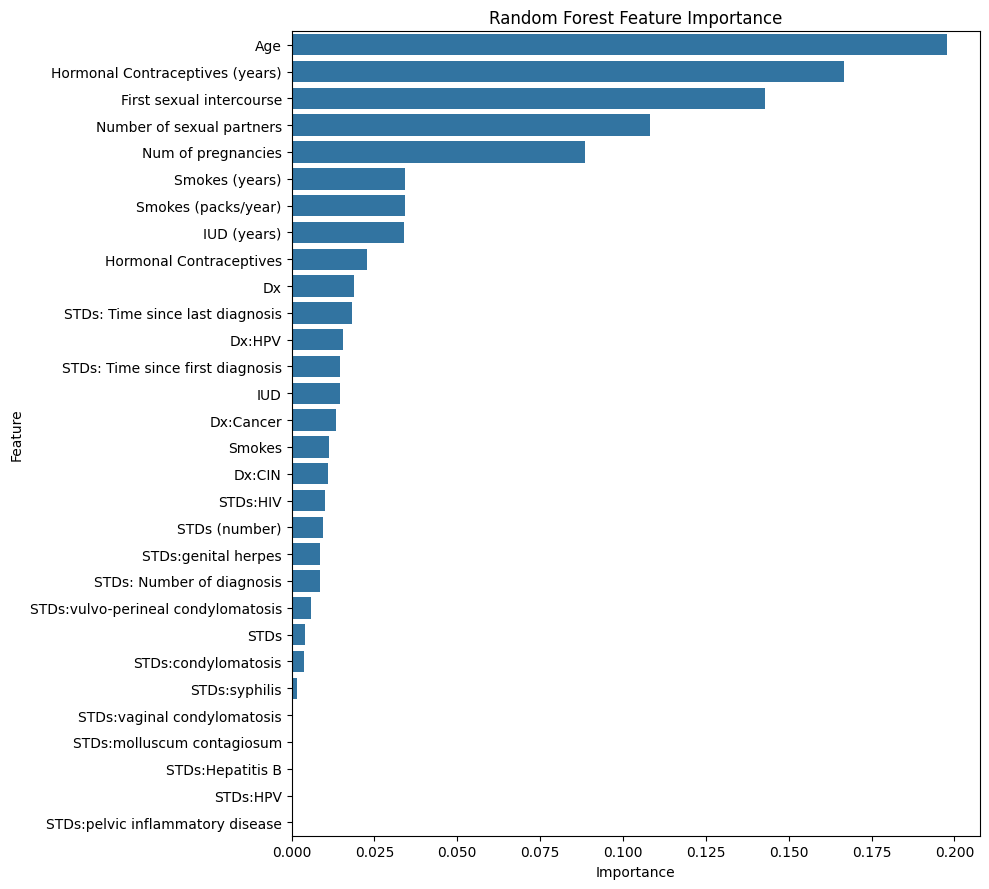
\includegraphics[width=\columnwidth]{rf_importance.png}
\caption{Random Forest impurity-based feature importance on the reconstructed
$858\times32$ frame, ranked in descending order. The Spearman rank correlation
with Figure~3 of the original study is $\rho=0.975$.}
\label{fig:rf-importance}
\end{figure}

\subsection{Model Architecture and Training}\label{sec:model}

\paragraph{Implementation environment of the original.} Several of the choices
described below rest on a hypothesis about the software used in the original
study, which we state explicitly so that it can be assessed independently. The
original reports a shallow network of 50 hidden neurons trained by scaled
conjugate gradient, and includes a training-progress figure of the form
produced by MATLAB's Neural Network Toolbox. We therefore treat that toolbox,
most plausibly through \texttt{patternnet} and \texttt{trainscg}, as the
working software hypothesis for the original implementation. This matters
because the toolbox applies several transformations by default that an author
would have no occasion to document. Wherever we adopt such a default, we
identify it as an inference drawn from this hypothesis rather than as a stated
procedure.

\paragraph{Architecture.} The network has 12 inputs, a single hidden layer of
50 units and a single output unit, with sigmoid activation at both layers as
specified in the original's Algorithm~1. Writing $\sigma$ for the logistic
function,
\begin{equation}
\sigma(z) = \frac{1}{1 + e^{-z}},
\label{eq:sigmoid}
\end{equation}
the network computes
\begin{align}
a^{(1)} &= \sigma\!\left(W^{(1)}x + b^{(1)}\right), \label{eq:hidden}\\
\hat{y} &= \sigma\!\left(W^{(2)}a^{(1)} + b^{(2)}\right), \label{eq:output}
\end{align}
with $W^{(1)} \in \mathbb{R}^{50 \times 12}$ and
$W^{(2)} \in \mathbb{R}^{1 \times 50}$. Predictions are obtained by
thresholding $\hat{y}$ at $0.5$.

The original's description of the output layer is not consistent across its
equations and figures. We therefore also evaluate a variant with
hyperbolic-tangent hidden activation and a two-unit softmax output,
corresponding to the toolbox defaults.

\paragraph{Initialisation.} Algorithm~1 specifies that weights are drawn from
$N(0,1)$ and bias nodes set to $1.0$, and we follow this exactly. A
Nguyen--Widrow-style initialisation, corresponding to the toolbox's
\texttt{initnw} alternative, is evaluated as a variant. This choice is not
incidental: because the derivative of the logistic function,
\begin{equation}
\sigma'(z) = \sigma(z)\bigl(1 - \sigma(z)\bigr),
\label{eq:sigmoid-deriv}
\end{equation}
attains a maximum of $0.25$ at $z=0$ and decays towards zero as $|z|$ grows,
the gradient available to the first layer is governed by the magnitude of the
pre-activations $W^{(1)}x + b^{(1)}$. Unit-variance weights applied to inputs
on their natural scales place those pre-activations far from the origin, as we
quantify below.

\paragraph{Input normalisation.} No scaling or normalisation step is described
anywhere in the original. We nonetheless apply min--max scaling of each input
to $[-1,1]$, corresponding to the toolbox's \texttt{mapminmax} default, which
is applied inside the training routine and would not ordinarily be reported by
an author. The scaler is fitted over all 858 rows, matching the toolbox
behaviour of normalising before its internal partition; fitting on the training
partition alone is retained as a sensitivity variant.

The consequences of omitting this step are severe. The input variables differ
by more than an order of magnitude in scale, from binary indicators to ages
ranging from 13 to 84, and the mean Euclidean norm of an input row is 32.9.
Under the initialisation of Algorithm~1 this yields hidden-layer
pre-activations with a standard deviation of 32.2, and 90.0\% of hidden-layer
activations fall below $0.01$ or above $0.99$ before any gradient step is
taken. By Equation~\eqref{eq:sigmoid-deriv} the mean sigmoid derivative in this
regime is $0.0102$, against a maximum of $0.25$. Holding the initial weights
fixed and rescaling the inputs alone, the pre-activation standard deviation
falls to 2.9, the saturated fraction to 17.3\%, and the mean derivative rises
to $0.0968$---a factor of approximately 9.5. Without normalisation the network
therefore begins training in a strongly saturated regime with heavily
attenuated gradients, which supplies a mechanistic account of the optimisation
difficulty we observe in its absence (Section~\ref{sec:ranking}).

\paragraph{Loss function.} The original specifies squared error in Algorithm~1
and reports minimised cross-entropy in its results section. We use binary
cross-entropy in the primary configuration and evaluate mean squared error as a
variant.

\paragraph{Training algorithm.} We implemented the scaled conjugate gradient
algorithm of M\o{}ller directly, including the finite-difference approximation
to the Hessian-vector product and the Levenberg--Marquardt-style scaling
parameter, rather than substituting a general-purpose conjugate gradient
routine; the latter performs a line search at each step and is a different
algorithm.

\begin{figure*}[t]
\centering
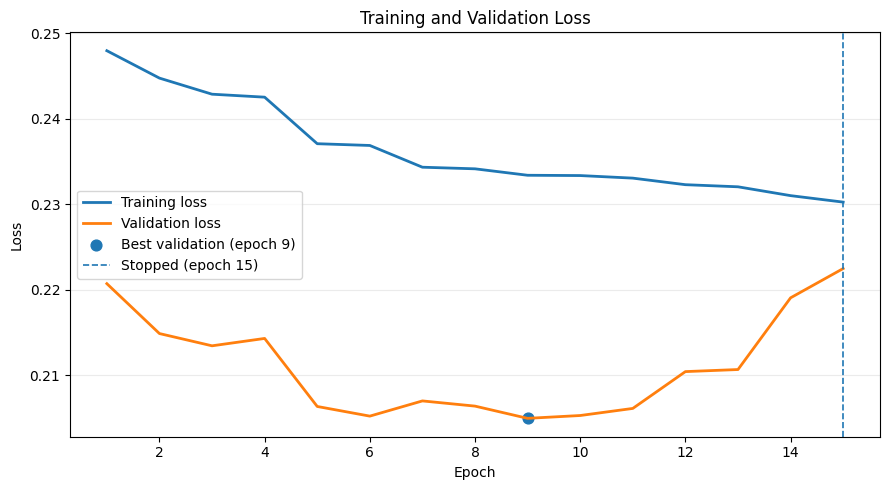
\includegraphics[width=0.78\textwidth]{loss_trajectory.png}
\caption{Training and validation loss for the primary configuration (twelve
features, sigmoid activation, cross-entropy loss, seed 42). Validation loss
attains its minimum at epoch~9 and training terminates at epoch~15 after six
consecutive increases. The corresponding figure in the original study shows a
best validation epoch of 3 and termination at epoch~9---the same interval of
six epochs. Note the vertical scale: training loss falls only from 0.248 to
0.230 across the full run, consistent with the attenuated gradients described
in Section~\ref{sec:model}.}
\label{fig:loss}
\end{figure*}

\paragraph{Stopping criterion.} The training duration is reported
inconsistently: the text states one epoch, while the accompanying training
figure shows nine. Rather than fixing the iteration count at either value, we
adopted the toolbox default of terminating after six consecutive increases in
validation loss, subject to a cap of 1000 epochs, and allowed training to halt
of its own accord. The stopping epoch is thereby an observation rather than an
assumption; Figure~\ref{fig:loss} shows the resulting trajectory.

\paragraph{Data partition.} The original reports a 70/15/15 split into
training, validation and test sets of 600, 129 and 129 observations. Neither
the random seed nor whether the split was stratified is reported. We used an
unstratified random split as an analogue of the toolbox's default random
division, with seed 42 in the primary run. This seed is our own choice and
carries no significance; the entire procedure is repeated across 30 seeds
(Figure~\ref{fig:seeds}) to establish that the behaviour reported below does
not depend on it. In the primary run the three partitions contain 40, 7 and 8
positive cases respectively.

\paragraph{Procedures not applied.} The original describes no class weighting,
resampling, synthetic oversampling or threshold adjustment, and we applied none
in the reproduced classifier. A Youden-optimal threshold is computed in
Section~\ref{sec:results} as a diagnostic only and forms no part of the
reproduction. We state this explicitly because each of these procedures would
materially alter the behaviour reported below, and their absence is a property
of the original design rather than of our reconstruction.

\paragraph{Configurations evaluated.} The ambiguities identified above admit
more than one defensible reading. Rather than selecting among them, we evaluate
the full factorial combination of feature set (ten or twelve variables),
architecture and loss (sigmoid with cross-entropy, sigmoid with squared error,
or tanh--softmax with cross-entropy) and initialisation ($N(0,1)$ or
Nguyen--Widrow), giving twelve configurations, each repeated across ten seeds.
Results for all twelve are reported in Section~\ref{sec:results}.

\begin{figure*}[t]
\centering
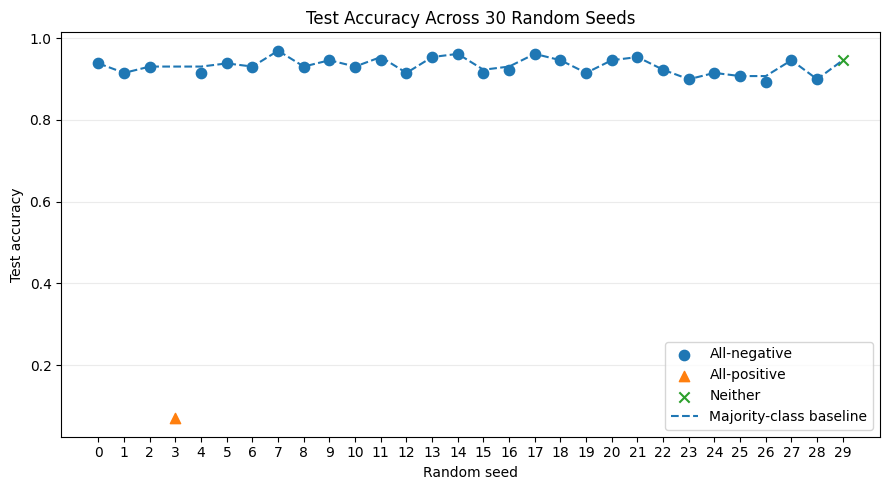
\includegraphics[width=0.78\textwidth]{seed_sweep.png}
\caption{Test accuracy across 30 random seeds, with points marked by the
behaviour of the resulting classifier. Twenty-eight runs assign every
observation to the negative class and attain accuracy equal to the
majority-class baseline of the corresponding split. One run (seed~3) assigns
every observation to the positive class, giving a true-positive rate and a
false-positive rate of 100\% at an accuracy equal to the positive prevalence of
its split. One run falls into neither category.}
\label{fig:seeds}
\end{figure*}

\subsection{Evaluation Protocol}\label{sec:eval}

\paragraph{Metric definitions.} We adopt the metric definitions given in the
original study. Writing TP, TN, FP and FN for the counts of true positives,
true negatives, false positives and false negatives,
\begin{align}
\mathrm{Accuracy} &= \frac{TP + TN}{TP + TN + FP + FN}, \label{eq:acc}\\[2pt]
\mathrm{TPR} &= \frac{TP}{TP + FN}, \label{eq:tpr}\\[2pt]
\mathrm{FPR} &= \frac{FP}{FP + TN}, \label{eq:fpr}\\[2pt]
\mathrm{FNR} &= \frac{FN}{FN + TP}. \label{eq:fnr}
\end{align}
We state these explicitly because the relations they impose are used in
Section~\ref{sec:results} to evaluate the internal consistency of the
originally reported figures. In particular,
Equations~\eqref{eq:tpr} and~\eqref{eq:fnr} give
$\mathrm{TPR} + \mathrm{FNR} = 1$ whenever the positive class is non-empty, and
for a confusion matrix with both classes represented these quantities are
uniquely determined. Precision, $TP/(TP+FP)$, and the $F_1$ score are reported
additionally; neither appears in the original.

\paragraph{The majority-class baseline.} Accuracy is not interpretable in
isolation on an imbalanced dataset, since it can be made large by ignoring the
minority class entirely. For each partition we therefore also report the
accuracy of the trivial classifier that assigns every observation to the more
frequent class, which is the larger of the two class proportions in that
partition. On the full dataset this quantity is 93.59\%. Every accuracy figure
reported in Section~\ref{sec:results} is accompanied by the corresponding
baseline and by the difference between the two, which we refer to as the lift
over baseline.

\paragraph{Threshold-free metrics.} The metrics above are computed from
thresholded predictions and therefore describe the classifier only at the
particular threshold applied. To characterise the model's ranking behaviour
independently of that choice, we additionally report the area under the
receiver operating characteristic curve (ROC-AUC) and the average precision
(AP), computed from the continuous network outputs.

The two require different reference points. ROC-AUC takes the value $0.5$ in
expectation for a classifier that ranks at random, irrespective of class
balance. Average precision does not share this property: for a random ranking
the expected average precision is the positive prevalence of the sample, here
$0.064$. An average precision figure is therefore reported alongside the
prevalence of the partition it was computed on, since the same numerical value
carries different meaning at different prevalences.

\paragraph{Metrics reported by the original.} The original reports accuracy,
mean squared error, true-positive rate, false-positive rate and false-negative
rate, together with a confusion matrix and a set of ROC curves. It does not
report the area under those curves, average precision, precision, $F_1$, any
majority-class baseline, or any measure of variability across repeated runs;
results are given for a single run whose random seed is not stated. Our
protocol reports the classification and threshold-free quantities given in the
original, except for the reported mean squared error, which we treat separately
because its calculation cannot be uniquely reconstructed from the published
information. We add the baseline comparison and the threshold-free metrics
described above.

\subsection{Software and Environment}\label{sec:software}

The reproduction was implemented in Python. The original is, under the software
hypothesis stated in Section~\ref{sec:model}, treated as a MATLAB
implementation; reimplementation in open-source software is therefore itself
part of this work, and any residual difference in numerical behaviour between
the two environments cannot be excluded as a source of discrepancy.

Data handling and preprocessing use \texttt{pandas} and \texttt{NumPy}. The
Random Forest of Section~\ref{sec:features} and all evaluation metrics use
\texttt{scikit-learn}. The network, the scaled conjugate gradient routine and
the initialisation schemes were implemented directly using \texttt{PyTorch}
tensors and automatic differentiation; no built-in optimiser was used. Figures
were produced with \texttt{Matplotlib} and \texttt{seaborn}. Package versions
are pinned in \texttt{requirements.txt} in the repository.

The stochastic components are seeded explicitly: the primary Random Forest uses
\texttt{random\_state=42}, while the data partition and neural-network
initialisation use the corresponding run seed. The primary run uses seed 42
throughout; the repetition analyses use seeds $0$ to $29$ and $0$ to $9$ as
described in Section~\ref{sec:model}. With fixed seeds and environment, the
implemented pipeline is intended to be reproducible, and re-execution
reproduces the figures and tables reported from the notebook.

The complete code, including the preprocessing rules, the sensitivity variants
and the scripts that generate each figure, is available at
\url{https://github.com/Prakhar-Sahu26/cervdetect-rescience}. The dataset is
not redistributed and is obtained directly from the UCI repository.

\section{Results}\label{sec:results}

\subsection{Reproduction of the Reported Confusion Matrix}\label{sec:cm}

The confusion matrices produced by the primary configuration are shown in
Figure~\ref{fig:confusion}. Across all three partitions the reproduced
classifier predicts the negative class for every observation: the training
partition yields 560 true negatives and 40 false negatives, the validation
partition 122 and 7, and the test partition 121 and 8. No observation in any
partition is assigned to the positive class, so the false-positive and
true-positive counts are zero throughout.

Pooling the three partitions gives 803 true negatives, 55 false negatives, and
no true or false positives across all 858 observations. This is identical, cell
for cell, to the confusion matrix reported in Figure~6 of the original study.
The per-partition counts differ slightly from those reported there---the
original gives 559 and 41 for training, and 123 and 6 for validation, against
our 560/40 and 122/7---but these differences reflect a different random
allocation of the same records between partitions, not a difference in
classifier behaviour. The test partition matches exactly at 121 and 8, and the
pooled totals are identical.

The reproduction therefore recovers the published classification behaviour
rather than approximating it. Both the published model and its reconstruction
assign every one of the 858 observations to the negative class, and neither
identifies any of the 55 biopsy-positive cases.

Training terminated at epoch~15, with the lowest validation loss attained at
epoch~9 (Figure~\ref{fig:loss}). The original's training figure shows a best
validation epoch of 3 and termination at epoch~9. The interval between the two
is six epochs in both cases, consistent with the stopping rule adopted in
Section~\ref{sec:model}. This also bears on the discrepancy noted earlier
between the original's text, which states one epoch, and its training figure,
which shows nine: under a stopping rule of six consecutive validation failures,
a figure terminating at epoch~9 is a total epoch count rather than a count of
training iterations, and the two statements cannot both describe the same
quantity.

\begin{figure}[!t]
\centering
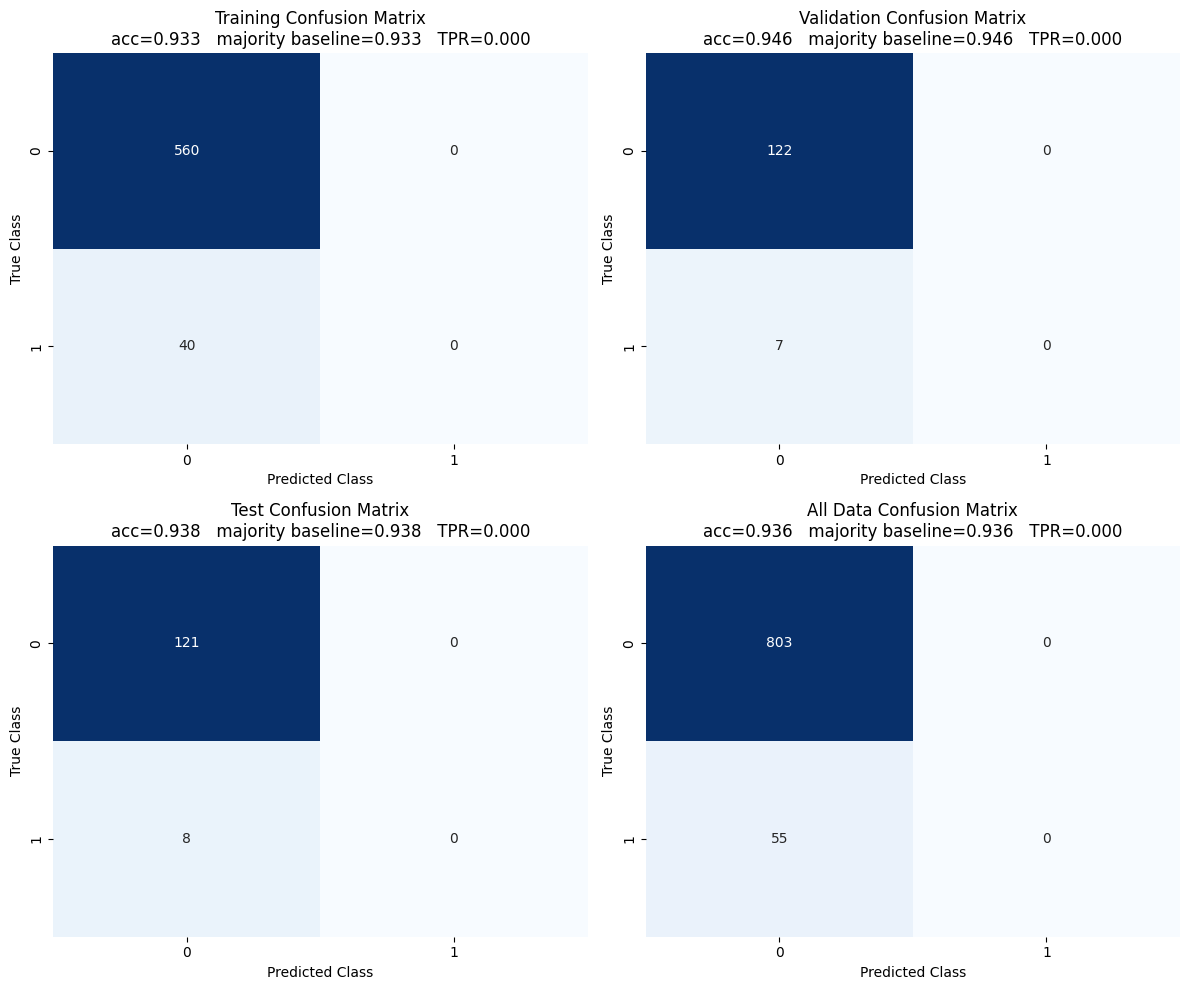
\includegraphics[width=\columnwidth]{confusion_matrix.png}
\caption{Confusion matrices for the primary configuration (twelve features,
sigmoid activation, cross-entropy loss, seed 42), by partition and pooled
across all 858 observations. In every panel the accuracy equals the
majority-class baseline of that partition and the true-positive rate is zero.
The pooled matrix is identical, cell for cell, to Figure~6 of the original
study.}
\label{fig:confusion}
\end{figure}

\subsection{Accuracy Relative to the Majority-Class Baseline}
\label{sec:baseline}

Table~\ref{tab:baseline} reports the accuracy of the reproduced classifier
alongside the majority-class baseline for each partition, as defined in
Section~\ref{sec:eval}.

In every partition the two quantities are equal and the lift over baseline is
zero. This follows directly from the confusion matrices of
Section~\ref{sec:cm}: a classifier that assigns every observation to the
negative class attains exactly the accuracy of the trivial classifier that does
the same, since the two make identical predictions on every record. The pooled
accuracy of 93.59\% is the negative-class prevalence of the dataset.

The original reports an accuracy of 93.6\% and does not report a baseline for
comparison. That figure agrees with both the accuracy of the reproduced
classifier and the accuracy attainable without reference to any input variable.

\begin{table}[t]
\centering
\footnotesize
\caption{Accuracy of the reproduced classifier against the majority-class
baseline, by partition. Lift is the difference between the two.}
\label{tab:baseline}
\renewcommand{\arraystretch}{1.2}
\begin{tabular}{@{}lrrrrr@{}}
\toprule
\textbf{Partition} & \textbf{$n$} & \textbf{Pos.} & \textbf{Accuracy}
& \textbf{Baseline} & \textbf{Lift} \\
\midrule
Training   & 600 & 40 & 0.9333 & 0.9333 & 0.0000 \\
Validation & 129 &  7 & 0.9457 & 0.9457 & 0.0000 \\
Test       & 129 &  8 & 0.9380 & 0.9380 & 0.0000 \\
\midrule
All data   & 858 & 55 & 0.9359 & 0.9359 & 0.0000 \\
\bottomrule
\end{tabular}
\end{table}

\subsection{Internal Consistency of the Originally Reported Metrics}
\label{sec:consistency}

The original reports classification metrics in three places: the abstract, the
results table (Table~4), and the confusion matrix (Figure~6). The values
implied by each are collected in Table~\ref{tab:consistency}.

The confusion matrix determines the remaining quantities uniquely. With
$TP = 0$, $FP = 0$, $FN = 55$ and $TN = 803$,
Equations~\eqref{eq:tpr}--\eqref{eq:fnr} give $\mathrm{TPR} = 0/55 = 0$,
$\mathrm{FPR} = 0/803 = 0$ and $\mathrm{FNR} = 55/55 = 1$, with an accuracy of
$803/858 = 0.9359$. The reported accuracy of 93.6\% agrees with this to the
precision given, as does the false-negative rate of 100\% reported in the
abstract.

The remaining reported values do not follow. Table~4 gives a true-positive rate
of 100\%, whereas the confusion matrix requires zero; the two are related by
$\mathrm{TPR} + \mathrm{FNR} = 1$, so a true-positive rate of 100\% and the
abstract's false-negative rate of 100\% cannot both hold. Table~4 further gives
a false-positive rate of 100\%, whereas the confusion matrix requires zero and
the abstract reports 6.4\% for the same quantity.

The value 6.4\% is consistent with a different quantity. The proportion of
misclassified observations is $(FP + FN)/n = 55/858 = 0.0641$, which agrees
with the reported figure to the precision given, whereas
Equation~\eqref{eq:fpr} applied to the published confusion matrix gives zero.

No assignment of values to $TP$, $TN$, $FP$ and $FN$ satisfies the metrics
reported in Table~4 and those reported in the abstract simultaneously. If the
three sources are intended to describe the same run at the same operating
point, their reported values are mutually incompatible, and at least one must
refer to a different result, contain an error, or arise from a different
calculation.

\begin{table}[t]
\centering
\footnotesize
\caption{Classification metrics as reported in three locations of the original
study, and as implied by its published confusion matrix. Dashes indicate
quantities not reported in that location.}
\label{tab:consistency}
\renewcommand{\arraystretch}{1.2}
\begin{tabular}{@{}lcccc@{}}
\toprule
\textbf{Source} & \textbf{Acc.} & \textbf{TPR} & \textbf{FPR} & \textbf{FNR} \\
\midrule
Abstract              & 93.6\% & ---    & 6.4\%  & 100\% \\
Table~4               & 93.6\% & 100\%  & 100\%  & ---   \\
Figure~6 (implied)    & 93.6\% & 0\%    & 0\%    & 100\% \\
\midrule
This reproduction     & 93.6\% & 0\%    & 0\%    & 100\% \\
\bottomrule
\end{tabular}
\end{table}

\subsection{Stability Across Random Initialisations}\label{sec:seeds}

The primary run reported above uses seed 42. To establish whether its behaviour
is characteristic of the pipeline or an artefact of that choice, the entire
procedure---partition, initialisation and training---was repeated across 30
seeds. Test accuracy for each run is shown in Figure~\ref{fig:seeds}, and the
distribution of test metrics is summarised in Table~\ref{tab:seeds}.

Twenty-eight of the 30 runs assign every observation to the negative class,
giving a true-positive rate of zero. The median true-positive rate across the
30 runs is $0.000$, with an interquartile range of $[0.000, 0.000]$; the median
$F_1$ score is likewise $0.000$. Median test accuracy is $0.930$, with an
interquartile range of $[0.915, 0.946]$, tracking the majority-class baseline
of each partition as the number of positive cases allocated to the test set
varies between 4 and 13.

The two remaining runs depart from this pattern in opposite directions. One
falls into neither category, recovering a small number of positive cases. The
other, seed~3, assigns every observation to the \emph{positive} class: on a
test partition containing 120 negative and 9 positive records it returns
$TP = 9$, $FP = 120$, $TN = 0$ and $FN = 0$, giving a true-positive rate of
100\%, a false-positive rate of 100\% and an accuracy of $9/129 = 0.070$, equal
to the positive prevalence of that partition. Training in this run terminated
at epoch~1 with the lowest validation loss recorded at epoch~0, indicating that
no trained epoch improved on the initial validation loss.

The all-negative outcome is therefore the typical behaviour of the pipeline
rather than a property of the particular seed used in the primary run. The
distribution of test metrics is also strongly affected by the small number of
positive cases available: across the 30 partitions the test set contains
between 4 and 13 positive records, so the recovery of a single additional
positive case changes the true-positive rate by between 8 and 25 percentage
points, and any recall figure derived from a single run carries substantial
variance.

\begin{table}[t]
\centering
\footnotesize
\caption{Distribution of test-set metrics across 30 random seeds.}
\label{tab:seeds}
\renewcommand{\arraystretch}{1.2}
\begin{tabular}{@{}lrrrr@{}}
\toprule
\textbf{Metric} & \textbf{Median} & \textbf{IQR} & \textbf{Min} & \textbf{Max} \\
\midrule
Accuracy          & 0.930 & [0.915, 0.946] & 0.070 & 0.969 \\
TPR               & 0.000 & [0.000, 0.000] & 0.000 & 1.000 \\
FNR               & 1.000 & [1.000, 1.000] & 0.000 & 1.000 \\
$F_1$             & 0.000 & [0.000, 0.000] & 0.000 & 0.222 \\
ROC-AUC           & 0.516 & [0.450, 0.577] & 0.273 & 0.739 \\
Average precision & 0.091 & [0.075, 0.123] & 0.039 & 0.176 \\
\midrule
\multicolumn{5}{@{}l}{Runs with $TP = 0$: 28 of 30} \\
\bottomrule
\end{tabular}
\end{table}

\subsection{Sensitivity to Ambiguous Implementation Choices}
\label{sec:sensitivity}

The results reported use a single reconstruction of the original pipeline.
Three of the ambiguities identified in Section~\ref{sec:methods} admit more
than one defensible reading: the size of the selected feature set, which the
original states as twelve but tabulates as ten; the architecture and loss
function, specified as sigmoid activation with squared error in Algorithm~1 but
reported as cross-entropy in the results section, with the toolbox defaults
implying a hyperbolic-tangent hidden layer and softmax output; and the
initialisation scheme, given as $N(0,1)$ in Algorithm~1 against the toolbox's
Nguyen--Widrow alternative. These give twelve reconstructions, each of which
follows the published description as closely as the description permits.

All twelve were evaluated over ten seeds. Median test metrics are reported in
Table~\ref{tab:grid}.

Every configuration returns a median true-positive rate of $0.000$. No
combination of feature set, architecture, loss function and initialisation
recovers any positive case at the median, and median accuracy lies between
$0.930$ and $0.934$ throughout, matching the majority-class baseline of the
test partition in each case.

The configurations are not otherwise equivalent. Median ROC-AUC ranges from
$0.425$ to $0.595$, and the median stopping epoch from 9 to 18.5, so the twelve
reconstructions produce measurably different models. On the twelve-feature set,
Nguyen--Widrow initialisation yields a higher median ROC-AUC than $N(0,1)$ in
all three architecture and loss pairings, by between $0.088$ and $0.155$; on
the ten-feature set the difference is smaller and not consistent in sign. Three
configurations return a median ROC-AUC below $0.5$. We do not identify any of
these configurations as the correct reconstruction, since the published
description does not determine which was used.

The variation in ranking behaviour therefore does not translate into any
variation in classification outcome. The all-negative result reported in
Sections~\ref{sec:cm} and~\ref{sec:seeds} does not depend on how the
ambiguities in the original description are resolved, and the inconsistencies
identified in the original text need not be settled in order to reproduce its
reported behaviour.

\begin{table}[t]
\centering
\footnotesize
\caption{Median test metrics across ten seeds for each of the twelve
reconstructions. V1: sigmoid hidden and output with binary cross-entropy.
V1b: as V1 with mean squared error. V2: hyperbolic-tangent hidden layer with
two-unit softmax output and cross-entropy.}
\label{tab:grid}
\renewcommand{\arraystretch}{1.15}
\begin{tabular}{@{}llrrrr@{}}
\toprule
\textbf{Features} & \textbf{Init.} & \textbf{Acc.} & \textbf{TPR}
& \textbf{AUC} & \textbf{Epoch} \\
\midrule
\multicolumn{6}{@{}l}{\emph{V1: sigmoid, cross-entropy}} \\
Twelve & $N(0,1)$ & 0.930 & 0.000 & 0.455 & 16.5 \\
Twelve & N--W     & 0.930 & 0.000 & 0.595 & 12.5 \\
Ten    & $N(0,1)$ & 0.930 & 0.000 & 0.474 & 14.0 \\
Ten    & N--W     & 0.930 & 0.000 & 0.480 & 11.0 \\
\midrule
\multicolumn{6}{@{}l}{\emph{V1b: sigmoid, squared error}} \\
Twelve & $N(0,1)$ & 0.930 & 0.000 & 0.425 & 15.0 \\
Twelve & N--W     & 0.930 & 0.000 & 0.580 & 14.0 \\
Ten    & $N(0,1)$ & 0.934 & 0.000 & 0.503 & 14.5 \\
Ten    & N--W     & 0.930 & 0.000 & 0.503 & 11.0 \\
\midrule
\multicolumn{6}{@{}l}{\emph{V2: tanh--softmax, cross-entropy}} \\
Twelve & $N(0,1)$ & 0.930 & 0.000 & 0.495 & 14.0 \\
Twelve & N--W     & 0.930 & 0.000 & 0.583 & 10.0 \\
Ten    & $N(0,1)$ & 0.930 & 0.000 & 0.489 & 18.5 \\
Ten    & N--W     & 0.930 & 0.000 & 0.444 & 9.0 \\
\bottomrule
\end{tabular}
\end{table}

\subsection{Ranking Behaviour and the Effect of Input Normalisation}
\label{sec:ranking}

The results above describe the classifier at the $0.5$ threshold. This section
examines the continuous outputs from which those predictions are derived, and
the effect of the normalisation step introduced in Section~\ref{sec:model}.

\paragraph{Effect of normalisation.} Without normalisation the network's
outputs are almost undifferentiated between classes: the difference in mean
predicted probability between biopsy-positive and biopsy-negative records is
$+0.0228$, and the difference in medians is $+0.0011$. Test ROC-AUC for that
run is $0.507$. With normalisation the median gap increases to $+0.0084$ and
test ROC-AUC to $0.583$. Average precision was not recorded for the
unnormalised run and is therefore not compared.

The normalised model also matches the original more closely, not less. The
unnormalised run recovers one positive case on the test partition, giving a
test confusion matrix of $TN=121$, $FP=0$, $FN=7$, $TP=1$; the normalised run
recovers none, reproducing the published matrix exactly
(Section~\ref{sec:cm}). An inferred preprocessing step that moves the
reconstruction towards the published result, rather than away from it, is
evidence that a comparable step was present in the original pipeline.

\paragraph{Threshold-free performance.} ROC-AUC and average precision for the
primary run are given in Table~\ref{tab:threshold-free}. Pooled across all 858
observations, ROC-AUC is $0.622$ and average precision $0.128$ against a
prevalence of $0.064$. Both exceed their reference values, so the model's
outputs carry some information about the target: ranking performance is above
the random-ranking reference, and average precision is roughly twice the
prevalence baseline.

That information does not survive thresholding. The distribution of predicted
probabilities by class is shown in Figure~\ref{fig:probs}. Positive records
receive slightly higher probabilities on average---mean $0.0883$ against
$0.0634$, median $0.0630$ against $0.0546$---but the two distributions show
substantial overlap. The highest probability assigned to any of the 858
observations is $0.4877$, and it belongs to a biopsy-negative record; the
highest assigned to any positive record is $0.4638$. Both fall below $0.5$, so
no observation can be classified positive at that threshold regardless of the
ranking information the outputs contain.

\paragraph{Threshold sensitivity.} The threshold maximising Youden's $J$ on the
test partition is $0.061$, close to the positive prevalence of the dataset. At
that threshold the classifier attains a true-positive rate of $0.625$ and a
false-positive rate of $0.331$, recovering five of the eight positive cases in
the test partition. This is reported as a diagnostic only; the reproduced
classifier uses the $0.5$ threshold throughout, as described in
Section~\ref{sec:model}.

\begin{table}[t]
\centering
\footnotesize
\caption{Threshold-free metrics for the primary run. Average precision is
compared against the positive prevalence of each partition, which is its
expected value under a random ranking.}
\label{tab:threshold-free}
\renewcommand{\arraystretch}{1.2}
\begin{tabular}{@{}lrrr@{}}
\toprule
\textbf{Partition} & \textbf{ROC-AUC} & \textbf{AP} & \textbf{Prevalence} \\
\midrule
Training   & 0.638 & 0.154 & 0.067 \\
Validation & 0.562 & 0.146 & 0.054 \\
Test       & 0.583 & 0.110 & 0.062 \\
\midrule
All data   & 0.622 & 0.128 & 0.064 \\
\bottomrule
\end{tabular}
\end{table}

\begin{figure}[!t]
\centering
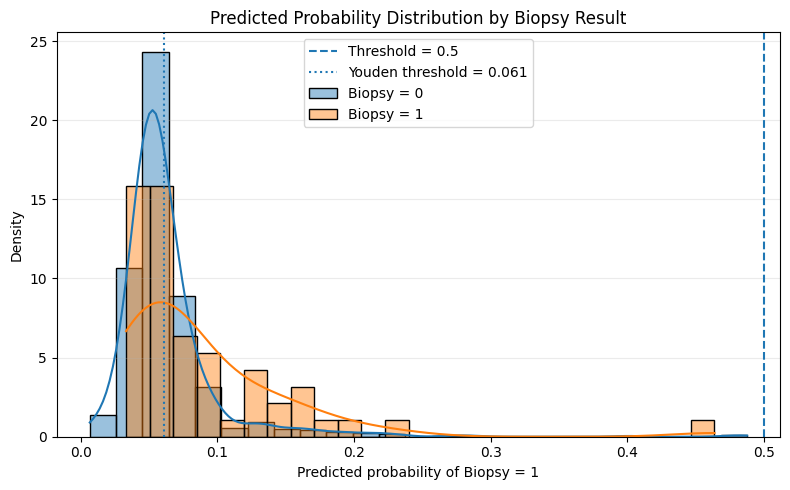
\includegraphics[width=\columnwidth]{probability_distribution.png}
\caption{Distribution of predicted probabilities by biopsy outcome, pooled
across all 858 observations. The dashed line marks the $0.5$ classification
threshold. No observation of either class receives a probability above
$0.4877$.}
\label{fig:probs}
\end{figure}

\section{Discussion}\label{sec:discussion}

\subsection{What Reproduces and What Does Not}\label{sec:what-reproduces}

The reconstructed pipeline reproduces the published confusion matrix, but not
all of the reported metrics, and these two outcomes are worth separating.

The confusion matrix reproduces exactly. Both the published matrix and ours
contain 803 true negatives, 55 false negatives, and no true or false positives
across all 858 observations. This agreement holds despite a reimplementation in
different software, an unreported random seed, and several points at which the
published description had to be interpreted
(Section~\ref{sec:sensitivity}). We therefore regard the published thresholded
prediction behaviour as successfully reproduced. Identical predictions do not
establish that the two implementations are identical in every internal respect,
but they do establish that the reported classification result is recoverable
from the published description.

What that classifier does is assign every observation to the negative class.
Its accuracy of $803/858 = 93.59\%$ is exactly the proportion of negative cases
in the dataset: the same accuracy is obtained by a classifier that ignores all
input variables and predicts the negative class for every observation. The
reproduction therefore recovers the original accuracy result while establishing
that the reported thresholded classifier provides no positive-case detection
beyond the majority-class baseline. Reproducibility and informativeness are
independent properties, and this study is an instance in which the first holds
and the second does not.

The reported metrics do not reproduce. The values in the original's Table~4
cannot be derived from its own published confusion matrix, and are inconsistent
with those reported in its abstract (Section~\ref{sec:consistency}). Our
reproduction agrees with the confusion matrix and with the abstract's
false-negative rate of 100\%, and disagrees with Table~4. If Table~4 and
Figure~6 are intended to describe the same run at the same operating point,
their reported values are mutually incompatible; this is a discrepancy internal
to the original rather than a disagreement between the original and this
reproduction. Whether they may instead describe different runs is considered in
Section~\ref{sec:metrics-discussion}.

A qualification is needed on what the network has learned. The all-negative
outcome invites the conclusion that it learned nothing, and this overstates the
case. Pooled ROC-AUC is $0.622$ and average precision $0.128$ against a
prevalence of $0.064$, so the continuous outputs exhibit weak discrimination
above the random-ranking reference. They show weak ranking ability rather than
the behaviour expected from a random ranking. They are nevertheless far too
weakly separated, at the reported operating point, to support a useful
diagnostic classifier: the two probability distributions show substantial
overlap, and no observation of either class receives a probability above
$0.4877$ (Section~\ref{sec:ranking}). The failure therefore does not imply an
absence of all signal; the continuous outputs exhibit weak ranking ability, but
under the reported $0.5$ threshold that signal does not produce any positive
prediction.

The appropriate interpretation is therefore not that the network learned
nothing, but that its weak continuous ranking signal does not translate into a
useful classifier at the reported threshold. The observed accuracy primarily
reflects the class distribution, whereas positive-class detection performance
is zero. The distinction between discrimination and thresholded classification
matters for interpreting what, if anything, can be salvaged from the approach,
which we examine in Section~\ref{sec:imbalance}.

\subsection{On the Reported Metrics}\label{sec:metrics-discussion}

Section~\ref{sec:consistency} established that the metrics reported in the
original's Table~4 cannot be derived from its published confusion matrix. This
section considers what might account for that.

The reported values are not arbitrary. A true-positive rate of 100\% together
with a false-positive rate of 100\% is the exact signature of a classifier that
assigns every observation to the positive class: such a classifier recovers
every positive case, giving $\mathrm{TPR} = TP/(TP+FN) = 1$, while
misclassifying every negative case, giving $\mathrm{FPR} = FP/(FP+TN) = 1$. The
pair of values reported in Table~4 is therefore not an arbitrary error but a
coherent description of a specific degenerate outcome---one that is the exact
class-prediction complement of the all-negative outcome shown in the same
paper's Figure~6.

That outcome is attainable under our reconstructed implementation of this
architecture. Among the 30 initialisations reported in
Section~\ref{sec:seeds}, one produced precisely this behaviour: on a test
partition of 120 negative and 9 positive records it returned $TN = 0$,
$FP = 120$, $FN = 0$ and $TP = 9$, giving a true-positive rate and a
false-positive rate of 100\% at an accuracy of $0.070$. Under our reconstructed
implementation the model can therefore collapse to either class depending on
initialisation, and both collapse modes were observed.

This suggests, but does not establish, that the original's Table~4 and Figure~6
describe different runs of an initialisation-sensitive model rather than a
single set of results. Under such a reading the accuracy of 93.6\% and the
false-negative rate of 100\% would derive from an all-negative run and the
true-positive and false-positive rates of 100\% from an all-positive one, which
would reconcile the reported values as originating from two different runs.

Three considerations bound what can be inferred from this. First, we cannot
observe the runs that produced the original's reported values, and no
combination of published information distinguishes this account from other
explanations, including transcription or tabulation error. Second, the
all-positive run we observed terminated at epoch~1, with the best validation
loss remaining at epoch~0; no trained epoch improved on the initial validation
loss. This run therefore does not establish that an all-positive classifier
would persist after successful optimisation. Third, the original also reports a
mean squared error of $0.07111$, but the published information does not allow
us to determine whether this value came from the same run as the reported
confusion matrix and rates.

We therefore report the correspondence as an observation rather than as an
explanation. What the reproduction establishes is narrower and does not depend
on the interpretation above: under the original's own stated definitions, the
reported metric values cannot jointly describe the same run as the published
confusion matrix. At least one reported value must therefore refer to a
different result, contain an error, or arise from a different calculation.
Determining which would require access to the original implementation.

\subsection{Obstacles to Reproduction}\label{sec:obstacles}

The reconstruction required decisions at points where the published description
did not determine an implementation. These are worth setting out, both because
they bound the confidence of the results above and because the categories they
fall into recur beyond this particular study.

\paragraph{Specifications that cannot be executed as written.} Two of the
original's imputation rules depend on one another for their inputs. Rule~4
derives the \emph{STDs} indicator from two individual disease columns, and
Rule~5 imputes those same columns by reference to \emph{STDs}. Because all
three columns share an identical missingness pattern, each rule requires as
input precisely the values the other produces, and no execution order satisfies
both (Section~\ref{sec:missing}). A reader cannot recover the intended
procedure from the text; we adopted the only order under which both rules have
defined inputs and recorded the deviation.

\paragraph{Quantities stated in a form that does not support the stated use.}
Rule~3 supplies two conditional proportions of the form
$P(\text{covariate} \mid \text{IUD})$, whereas imputing the IUD variable
requires $P(\text{IUD} \mid \text{covariate})$. No base rate is given by which
to invert them, and no assignment rule is stated. We evaluated three candidate
readings against the records with observed IUD status; the best agreed with
74.9\% of them, so approximately a quarter of the 117 imputed values are
expected to be incorrect under any available reading. This is the largest
single source of uncertainty in the reconstruction.

\paragraph{Steps performed but not described.} The variable \emph{STDs:HIV}
appears in the original's Figure~2 and therefore appears to have been retained
through preprocessing, but no rule anywhere in the text addresses it. Input
normalisation is a more consequential instance: no scaling step is described,
yet without one the network begins training in a strongly saturated regime with
heavily attenuated gradients (Section~\ref{sec:model}). Both steps are
plausible components of the pipeline that produced the published results, but
neither procedure is explicitly recoverable from the paper.

\paragraph{Internally inconsistent statements.} The original specifies squared
error in Algorithm~1 and reports cross-entropy in its results section; states
that twelve features were used while tabulating ten; states one training epoch
while its training figure shows nine; and reports three mutually incompatible
sets of classification metrics. Each of these required us to select a reading.

\paragraph{Undetermined parameters.} Random Forest hyperparameters, all random
seeds, and whether the data partition was stratified are not reported. These
omissions prevent exact reconstruction of any particular original run. The
random initialisation is especially consequential here, since our 30-seed
analysis produced qualitatively different collapse modes
(Section~\ref{sec:seeds}); the unreported Random Forest settings appear less
consequential for reproducing the published feature ranking, since the
resulting ranking agreed closely with the published one under our default
reconstruction.

\paragraph{Consequences.} These obstacles had markedly different effects. The
alternative interpretations we evaluated did not change the outcome: median
true-positive rate remained $0.000$ and median accuracy remained at the
majority-class baseline across all twelve configurations
(Section~\ref{sec:sensitivity}), so the central qualitative conclusion is
recoverable without resolving these internal inconsistencies. The undocumented
normalisation step was by contrast decisive, in that omitting it changes the
optimisation regime substantially. The circular imputation rules and the IUD
specification affect the reconstructed dataset itself, and their effects cannot
be fully quantified from the published information.

It is worth noting which of these mattered least. The inconsistencies most
visible on reading the paper---the feature count, the loss function, the epoch
count---did not alter the qualitative conclusion under any interpretation we
tested. Among the ambiguities we evaluated, the step with the clearest effect
on optimisation behaviour was one the paper does not mention. This asymmetry
suggests that completeness of description bears more directly on
reproducibility than internal consistency: a reader can adjudicate between two
stated alternatives, but cannot recover a step that was never stated.

\subsection{Evaluation Under Class Imbalance}\label{sec:imbalance}

The dataset used here contains 55 positive cases among 858 records, a positive
prevalence of 6.41\%. At that prevalence a classifier that predicts the
negative class for every observation attains 93.59\% accuracy, and this is what
the original reports.

The difficulty is not that accuracy is a poor metric in general, but that on
imbalanced data it is uninterpretable without a reference point. The reported
figure of 93.6\% is compatible with a model that has learned a useful
relationship and with one that ignores its inputs entirely, and nothing in the
number itself distinguishes the two. Reporting the majority-class baseline
alongside resolves this at no cost: the difference between the two values is
the quantity that carries information about the model, and here it is zero on
every partition (Section~\ref{sec:baseline}).

Three further reporting practices would have made the behaviour visible in this
case. Sensitivity and specificity, or an explicit confusion matrix, distinguish
performance on the two classes---the original does publish a confusion matrix,
and it is from that matrix rather than from the reported metrics that the
model's behaviour can be determined. Threshold-free metrics separate ranking
ability from classification: here they show weak discrimination that the
reported operating point does not exploit
(Section~\ref{sec:ranking}). Repeated runs establish whether a reported result
is characteristic or incidental; a single run of this pipeline could have
produced either collapse mode (Section~\ref{sec:seeds}).

The choice of decision threshold deserves particular attention. A threshold of
$0.5$ is a default rather than a principled choice, and under strong imbalance
it is often the wrong one. In our reproduction the threshold maximising
Youden's $J$ on the test partition was $0.061$, close to the positive
prevalence, at which the classifier recovered five of eight positive cases at a
false-positive rate of $0.331$. That operating point is not obviously
appropriate for deployment either, but the difference between it and the
reported one is substantial, and the original does not report a threshold or
indicate that any alternative was considered.

None of this is specific to the study reproduced here. The combination of a
rare positive class, accuracy as the headline metric, no baseline comparison,
and an unexamined default threshold is common enough that it forms a
recognisable pattern, and it produces results that are simultaneously
reproducible and uninformative. The corrective is inexpensive: a baseline
figure alongside every accuracy, a threshold-free metric reported with its
reference value, and some indication of variability across runs.

\subsection{Clinical Implications}\label{sec:clinical}

The reproduced classifier is not suitable for diagnostic or screening use at
the operating point reported. It attains 93.6\% accuracy while assigning every
observation to the negative class, giving a sensitivity of zero and a
false-negative rate of 100\%: all 55 biopsy-positive records in the dataset are
classified as negative.

The asymmetry of costs in screening makes this more consequential than the
accuracy figure suggests. A false positive typically results in further
testing, which carries cost and anxiety but is recoverable. A false negative is
a missed case, and in cervical cancer specifically the value of screening rests
on detection at a stage when intervention is effective. A model that identifies
no positive cases provides nothing that the decision to screen is intended to
provide.

The reported false-positive rate warrants comment for the same reason. A
false-positive rate of zero appears favourable in isolation, but it is attained
here trivially, by never predicting the positive class, and is achieved
together with a false-negative rate of 100\%. In a screening context the two
quantities cannot be assessed independently: any classifier can drive either to
zero by ignoring the corresponding class, and a low false-positive rate is
informative only alongside a sensitivity that is not zero.

This does not imply that the underlying data are uninformative or that the
approach is without value. The continuous outputs discriminate weakly above the
random-ranking reference (Section~\ref{sec:ranking}), and at a threshold
matched to the positive prevalence the same model recovers five of eight
positive cases in the test partition, albeit at a false-positive rate of
$0.331$. What the reproduction establishes is narrower: that the classifier as
reported, at the threshold reported, detects no positive cases, and that its
headline accuracy reflects the class distribution rather than any diagnostic
capability.

\subsection{Limitations}\label{sec:limitations}

Several limitations bound the conclusions above.

\paragraph{The software hypothesis is unverified.} Our treatment of input
normalisation, the stopping rule and the alternative architecture and
initialisation variants rests on the hypothesis that the original was
implemented in MATLAB's Neural Network Toolbox
(Section~\ref{sec:model}). This is inferred from the reported training
algorithm, network size and the form of the published training figure, and is
supported by the agreement between our stopping behaviour and the original's,
but it is not established. If the original used different software, the
defaults we adopted may not correspond to what was applied.

\paragraph{No individual original run can be reproduced.} Random seeds, Random
Forest hyperparameters and the stratification of the data partition are not
reported, so our results describe the distribution of outcomes the pipeline
produces rather than the particular run the original reports. Given the
variation across initialisations documented in Section~\ref{sec:seeds}, this is
a material limitation on any comparison at the level of a single number.

\paragraph{The reconstructed dataset is not certain to match the original.}
Approximately a quarter of the 117 imputed IUD values are expected to be
incorrect under the best available reading of Rule~3
(Section~\ref{sec:missing}), and the circular dependency between Rules~4 and~5
was resolved by a choice the original does not specify. The dataset on which
our model was trained therefore differs from the original's by an unknown
amount. The close agreement of the feature-importance ranking
($\rho = 0.975$) suggests the difference is small, but does not bound it.

\paragraph{Feature selection precedes the data partition.} We retained the
pipeline order given in the original, in which the Random Forest ranking is
computed on all 858 records including those later allocated to the test
partition (Section~\ref{sec:features}). This constitutes information leakage
from the test partition, and the test metrics we report are correspondingly
optimistic; an unbiased evaluation would therefore be expected to perform no
better. We additionally ran a split-first variant in which every imputation
statistic, the Random Forest ranking and the scaler were fitted on the training
partition alone. The classification behaviour was unchanged: the leak-free
pipeline also assigns every test observation to the negative class. The
inherited leakage therefore does not account for the reported result. The
leak-free feature ranking does differ from the original-faithful one, since it
is fitted on 600 records rather than 858. That variant is not itself a
reproduction of the original, which specifies the leaky ordering.

\paragraph{The reported mean squared error is not evaluated.} Because the
original specifies squared error in one place and cross-entropy in another, we
could not determine which quantity its reported value of $0.07111$ refers to,
and did not attempt a comparison (Section~\ref{sec:eval}).

\paragraph{Repetition counts are modest.} The stability analysis uses 30 seeds
and the configuration grid ten seeds per cell. These are sufficient to
establish that the all-negative outcome is typical rather than incidental, but
not to characterise the tails of the distribution: the single all-positive run
observed gives an estimated frequency with a wide interval, and we do not
report confidence intervals on any of the aggregate metrics.

\paragraph{Scope.} This is a reproduction of one study. The reporting practices
discussed in Section~\ref{sec:imbalance} recur widely, but we have not surveyed
the literature systematically and make no quantitative claim about their
prevalence.

\section{Conclusion}\label{sec:conclusion}

We reimplemented the CervDetect pipeline from its published description and
reproduced the confusion matrix reported in the original study exactly: 803
true negatives, 55 false negatives, and no true or false positives across all
858 observations. The reproduced classifier assigns every record to the
negative class. Its accuracy of 93.6\% is the proportion of negative cases in
the dataset, obtainable by a classifier that ignores every input variable, and
its sensitivity is zero.

The reported metrics are not internally consistent. Under the original's own
stated definitions, the values given in its Table~4 cannot jointly describe the
same run as its published confusion matrix, and at least one reported figure
must refer to a different result, contain an error, or arise from a different
calculation.

The behaviour we observe is not an artefact of our reconstruction. It persists
across 30 random initialisations and across all twelve interpretations of the
original's ambiguous implementation details that we evaluated. Among the
ambiguities we evaluated, the step with the clearest effect on optimisation
behaviour was one the paper does not describe at all.

The reproduction nonetheless has continuing use. The implementation is openly
available and fully specified, including the resolutions adopted for each
ambiguity in the original description, and provides a reference against which
alternative preprocessing, class-imbalance handling, threshold selection or
model choices can be compared on this dataset. Its continuous outputs
discriminate weakly above the random-ranking reference, so the pipeline is a
starting point for such comparisons rather than a dead end.

The reported accuracy is therefore reproducible but uninformative, and the
study's detection claims are not supported by its own results. Reporting a
majority-class baseline alongside accuracy, a threshold-free metric with its
reference value, and some measure of variability across runs would have made
this visible in the original.

\section*{Declaration}

\noindent\textbf{Conflict of Interest.} The authors declare no conflict of
interest.

\vspace{0.5em}
\noindent\textbf{Funding.} This research received no specific grant from any
funding agency in the public, commercial or not-for-profit sectors.

\vspace{0.5em}
\noindent\textbf{Author Contribution.} P.~Sahu: conceptualisation,
methodology, software, formal analysis, investigation, visualisation, writing
--- original draft. P.~Sudele: validation, writing --- review and editing.

\vspace{0.5em}
\noindent\textbf{Data Availability.} This study uses the Cervical Cancer
(Risk Factors) dataset, publicly available from the UCI Machine Learning
Repository~\cite{fernandes2017}. No new data were generated.

\vspace{0.5em}
\noindent\textbf{Code Availability.} The complete implementation, including
the preprocessing rules, the resolutions adopted for each ambiguity in the
original description, the sensitivity variants and the code generating each
figure and table, is available at
\url{https://github.com/Prakhar-Sahu26/cervdetect-rescience}.

\vspace{0.5em}
\noindent\textbf{Use of Generative AI.} Generative AI tools (OpenAI GPT and
Anthropic Claude) were used during the preparation of this work for debugging
code, checking factual details and reviewing draft text. All analyses,
implementation decisions and reported results were produced and verified by the
authors, who take full responsibility for the content of this manuscript.

\vspace{0.5em}
\noindent\textbf{Acknowledgements.} We thank the authors of the original study
for describing their methodology in sufficient detail to permit this
reproduction, and Kartik Chouksey for proofreading and review, which identified
gaps and improved the consistency of the manuscript.
